\section{Objectives}
Rebuild the Lab 19 supply IR-drop and decoupling comparison from PDF pages 78--80, including the peak-current explanation and capacitor costs.

\section{Specification Mapping}
S denotes simulated checks; D denotes analytical discussion.

\small\begin{longtable}{p{.46\linewidth}p{.30\linewidth}p{.15\linewidth}}\toprule
Requirement and PDF pages & Deck / check & Status \\ \midrule\endhead
Fig.19.1 four stages and two 1-ohm resistors (78,80) & D01/C0 & S \\
Observe external/internal rails and R1/R2 currents (78,80) & D01; printed traces & S \\
10pF/100pF/1nF comparison (79--80) & D01/C1--3 & S \\
Peak current, costs and use cases (80) & Results/discussion & S+D \\
\bottomrule\end{longtable}\normalsize


\section{Circuit and Design Derivation}
Four inverter stages have multipliers 30,60,180,540 with unit $W_p/W_n/L=3.6/1.8/0.25\,\mu$m. A 1 $\Omega$ resistor connects each external supply/return to its internal rail. The final stage additionally drives 10 fF to internal ground. Decoupling connects internal VDD to internal ground; it is not attached across the ideal external source. $10^{-21}$ F approximates no added capacitor.
\[\Delta V_R=IR,\qquad i_C=C\,d(V_{DD,int}-V_{GND,int})/dt.\]
This is a lumped-RC supply model without extracted metal or package inductance.

\section{Simulation Setup}
The model is supplied separately on the user's computer. These are 1 V, 27 $^\circ$C teaching conditions; the handout's old-process 2.5 V numbers are not pass thresholds. Actual PrimeSim HSPICE S-2021.09 runs use \texttt{accurate}, \texttt{runlvl=5} and \texttt{.print/.measure} data. Every \texttt{.alter} resets baseline parameters and temperature. All cases completed without errors or failed measurements; model and convergence notices may remain. Public netlists retain only \texttt{* MODEL\_SETUP\_REQUIRED}, with no model path. Full data are under the lab's \texttt{results/}; large files are split by deck and indexed by \texttt{simulation\_data.json}.

One deck contains four cases. The 0--1 V input uses 50 ps edges, 1 ns delay, 2 ns high time and a 4 ns period. Simulation lasts 20 ns with at most 2 ps steps. All summaries use the same 4--20 ns observation window.

\section{Results and Specification Checks}
\begin{center}\small\begin{tabular}{lrrrrr}\toprule
C & $V_{rail,min}$ & $\Delta V_{rail,pp}$ & $I_{R1,pk}$ & $I_{R2,pk}$ & $P_{avg}$ \\ \midrule
0 & 0.93453 & 63.350 & 32.734 & 32.738 & 9.923 \\
10 pF & 0.93486 & 62.301 & 32.570 & 32.573 & 9.930 \\
100 pF & 0.94510 & 50.913 & 27.447 & 27.449 & 9.975 \\
1 nF & 0.96779 & 23.425 & 17.507 & 17.283 & 9.520 \\
\bottomrule\end{tabular}\end{center}
Minimum rail voltage is in volts; rail peak-to-peak ripple in mV; currents in mA; power in mW. Minimum differential supply rises from 0.93453 V without decoupling to 0.96779 V at 1 nF. R1 peak current falls from 32.734 to 17.507 mA, with a similar R2 trend. The small improvement at 10 pF shows that capacitance must be evaluated relative to switched charge.
\begin{figure}[htbp]\centering
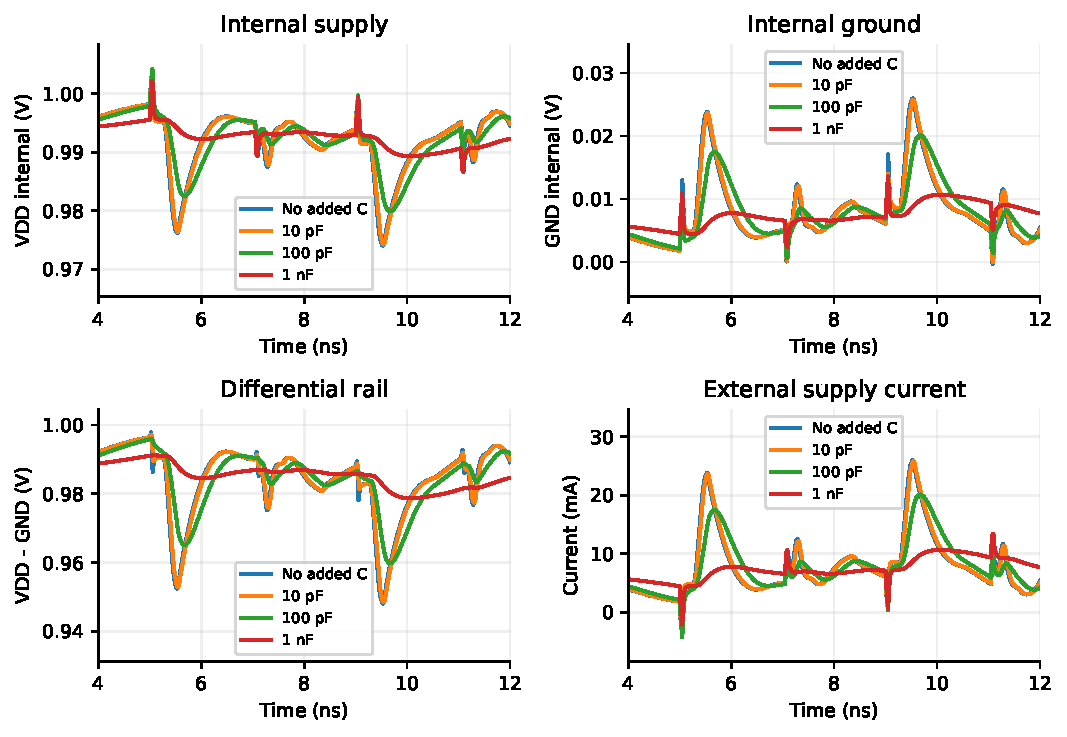
\includegraphics[width=\linewidth]{figures/supply_decoupling.pdf}
\caption{Actual internal supply, ground, differential rail and source current. The figure zooms to 4--12 ns; summaries use all of 4--20 ns.}
\end{figure}


\section{Discussion}
During rapid switching, the capacitor supplies or absorbs local charge and smooths current through the external resistors, reducing peak voltage drop. It does not remove average DC IR drop. Larger capacitance improves transient supply but consumes physical area and increases charging/startup time; real devices also have leakage, ESR/ESL and fabrication constraints. No physical area is inferred from an ideal capacitor value.

Decoupling need depends on allowable noise, simultaneous switching and supply impedance. Improving supply routing or staggering switching can also help; local fast current loads motivate local capacitance. Finite-window average power must not be equated with peak-current reduction: capacitor charging and initial conditions also affect the average.

\section{Conclusion}
All four capacitor conditions and both supply branches were simulated. A 1 nF capacitor substantially reduces differential rail ripple, without making the rails perfectly fixed or providing physical power-integrity signoff.
